% VLDB template version of 2020-08-03 enhances the ACM template, version 1.7.0:
% https://www.acm.org/publications/proceedings-template
% The ACM Latex guide provides further information about the ACM template

\documentclass[sigconf,nonacm,screen]{acmart}

\usepackage{listings}
\usepackage{algorithm}
\usepackage{algpseudocode}
\usepackage{float}
%\usepackage{balance}
\floatstyle{plaintop}
\restylefloat{table}

\renewcommand{\algorithmicrequire}{\textbf{Input:}}
\renewcommand{\algorithmicensure}{\textbf{Output:}}
\renewcommand{\algorithmiccomment}[1]{\hfill \textit{// #1}}

%\usepackage{fontawesome}
\newcommand{\eg}{e.\,g.,\ }
\newcommand{\ie}{i.\,e.,\ }
\usepackage{csquotes} %\enquote{}

%% The following content must be adapted for the final version
% paper-specific
\newcommand\vldbdoi{XX.XX/XXX.XX}
\newcommand\vldbpages{XX-XX}
% issue-specific
\newcommand\vldbvolume{17}
\newcommand\vldbissue{1}
\newcommand\vldbyear{2024}
% should be fine as it is
\newcommand\vldbauthors{\authors}
\newcommand\vldbtitle{\shorttitle} 
% leave empty if no availability url should be set
\newcommand\vldbavailabilityurl{https://github.com/damslab/reproducibility}
% whether page numbers should be shown or not, use 'plain' for review versions, 'empty' for camera ready
\newcommand\vldbpagestyle{plain} 

\newcommand{\mat}[1]{\ensuremath{\mathbf{#1}}}
\newtheorem{example2}{Example}
\newcommand{\card}[1]{\lvert #1\rvert}


\begin{document}
\title{POLAR: Adaptive and Non-invasive Join Order Selection via Plans of Least Resistance}

%%
%% The "author" command and its associated commands are used to define the authors and their affiliations.
\author{David Justen}
\affiliation{\institution{TU Berlin}}
%\email{david.justen@tu-berlin.de}
%\orcid{1234-5678-9012}
\authornote{Work started during time at Hasso Plattner Institute \cite{DBLP:journals/sigmod/PerscheidPRST22}}

\author{Daniel Ritter}
\affiliation{\institution{SAP}}
%\email{daniel.ritter@sap.com}
%\orcid{0000-0001-6146-3365}
\authornotemark[1]

\author{Campbell Fraser}
\affiliation{\institution{Google}}
%\email{campbellf@google.com}

\author{Andrew Lamb}
\author{Nga Tran}
\affiliation{\institution{InfluxData}}
%\email{alamb@influxdata.com}
%\email{ntran@influxdata.com}

\author{Allison Lee}
\affiliation{\institution{Snowflake}}
%\email{allison.lee@snowflake.com}

\author{Thomas Bodner}
\affiliation{\institution{Hasso Plattner Institute,}\institution{University of Potsdam}}
%\email{thomas.bodner@hpi.de}
%\orcid{0000-0002-7822-2098}

\author{Mhd Yamen Haddad}
\affiliation{\institution{INRIA, Ecole Polytechnique}}
%\email{mhaddad@yugabyte.com}
%\orcid{0000-0002-2206-1328}

\author{Steffen Zeuch}
\author{Volker Markl}
\affiliation{\institution{TU Berlin}}

\author{Matthias Boehm}
\affiliation{\institution{TU Berlin}}
%\email{matthias.boehm@tu-berlin.de}

%%
%% The abstract is a short summary of the work to be presented in the
%% article.
\begin{abstract}
%1. State the problem
Join ordering and query optimization are crucial for query performance but remain challenging due to unknown or changing characteristics of query intermediates, especially for complex queries with many joins.
%2. Say why it's an interesting problem
Over the past two decades, a spectrum of techniques for adaptive query processing (AQP)---including inter-/intra-operator adaptivity and tuple routing---have been proposed to address these challenges. However, commercial database systems in practice do not implement holistic AQP techniques because they increase the system complexity (e.g., intertwined planning and execution) and thus complicate debugging and testing. Additionally, existing approaches may incur large overheads, leading to problematic performance regressions.
%3. Say what your solution achieves
In this paper, we introduce POLAR, a simple yet very effective technique for a self-regulating selection of alternative join orderings with bounded overhead. We enhance left-deep join pipelines with alternative join orders, perform regret-bounded tuple routing to find and validate \enquote{plans of least resistance}, and then process the majority of tuple batches through these plans. We study different join order selection techniques, different routing strategies, and a variety of workload characteristics.
%4. Say what follows from your solution
Our experiments with a POLAR prototype on DuckDB show runtime improvements of up to 9x compared to non-adaptive pipelines and up to 74x compared to state-of-the-art AQP systems. With tuned exploration budgets, POLAR shows no more than 5\% overhead compared to DuckDB. 

\end{abstract}

\maketitle

%%% do not modify the following VLDB block %%
%%% VLDB block start %%%
\pagestyle{\vldbpagestyle}
\begingroup\small\noindent\raggedright\textbf{PVLDB Reference Format:}\\
\vldbauthors. \vldbtitle. PVLDB, \vldbvolume(\vldbissue): \vldbpages, \vldbyear.\\
\href{https://doi.org/\vldbdoi}{doi:\vldbdoi}
\endgroup
\begingroup
\renewcommand\thefootnote{}\footnote{\noindent
This work is licensed under the Creative Commons BY-NC-ND 4.0 International License. Visit \url{https://creativecommons.org/licenses/by-nc-nd/4.0/} to view a copy of this license. For any use beyond those covered by this license, obtain permission by emailing \href{mailto:info@vldb.org}{info@vldb.org}. Copyright is held by the owner/author(s). Publication rights licensed to the VLDB Endowment. \\
\raggedright Proceedings of the VLDB Endowment, Vol. \vldbvolume, No. \vldbissue\ %
ISSN 2150-8097. \\
\href{https://doi.org/\vldbdoi}{doi:\vldbdoi} \\
}\addtocounter{footnote}{-1}\endgroup
%%% VLDB block end %%%

%%% do not modify the following VLDB block %%
%%% VLDB block start %%%
\ifdefempty{\vldbavailabilityurl}{}{
\vspace{.3cm}
\begingroup\small\noindent\raggedright\textbf{PVLDB Artifact Availability:}\\
The source code, data, and/or other artifacts have been made available at \url{\vldbavailabilityurl}.
\endgroup
}
%%% VLDB block end %%%

%% INTRODUCTION
\section{Introduction}

\begin{figure*}[t]
    \centering
    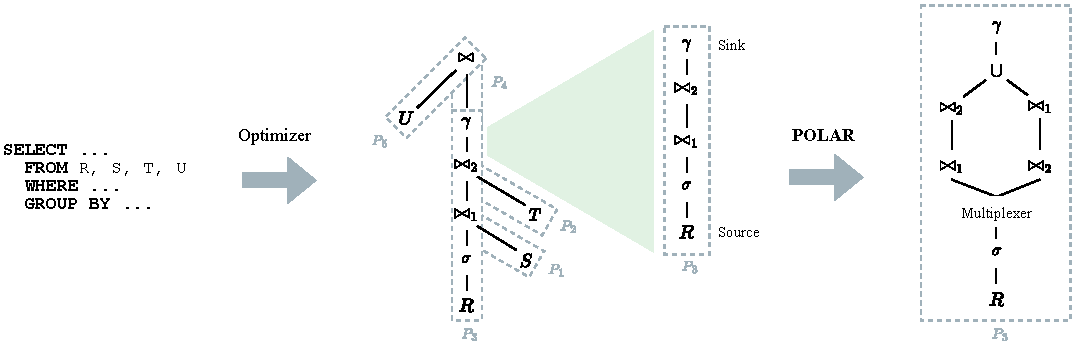
\includegraphics[width=0.9\textwidth]{figures/polar_pipeline-4.pdf}
		\vspace{-0.5cm}
		\caption{POLAR pipeline compilation from input query via standard, pipelined plan to POLAR pipelines.}
    \label{fig:pipeline_design}
		\vspace{-0.1cm}
\end{figure*}

% context
Cost-based query optimizations \cite{SelingerACLP79,moerkotte23} for selecting optimal join orders, join methods, and data access paths are crucial for the end-to-end performance of analytical queries. State-of-the-art exact join ordering algorithms such as DPsize~\cite{SelingerACLP79,HanKLLM08}, DPsub, DPcpp~\cite{MoerkotteN06}, and DPhyp~\cite{MoerkotteN08} rely on dynamic programming for efficient enumeration and are agnostic to used cost model and cardinality estimates. These algorithms yield optimal execution plans, but only under the assumption of precise cardinality estimates. 

\textbf{Cardinality Estimation Challenges:} Estimating precise cardinalities for intermediate results of complex queries remains a stubbornly difficult problem~\cite{LeisGMBK015}. Inaccuracies stem from multiple sources. First, most systems assume uniform distributions (no skew) and independence of predicates (no correlation) \cite{IlyasMHBA04}. These simplifying assumptions often cause under-estimation, which is problematic due to plan choices with poor asymptotic behavior~(\eg nested-loop joins), which perform poorly for larger intermediates \cite{IlyasMHBA04,LeisGMBK015}. Second, missing or too coarse-grained statistics (\eg histograms \cite{KanneM10} or sketches \cite{IzenovDRS21}) can cause deviations for clustered data. Third, user-defined functions and new environments (\eg cloud, federated, raw data) often do not allow obtaining statistics \cite{HueskePSRBKT12,JosifovskiSHL02,ReyFN23}. Fourth, complex queries with many operators are difficult to estimate because errors propagate exponentially \cite{IzenovDRS21,IoannidisC91,MoerkotteNS09}. Although recent work on ML-based estimators \cite{KipfKRLBK19,DuttWNKNC19,YangLKWDCAHKS19}, learning to distrust certain estimates \cite{MarcusNMZAKPT19}, and learning to rank plans \cite{BehrMK23} offer benefits, they do not solve all problems above.

\textbf{Adaptive Query Processing (AQP):} In the past two and a half decades, a spectrum of AQP techniques \cite{BabuB05,DeshpandeIR07,IvesDR07,DeshpandeHR06} has been devised to address the challenges of unknown and changing data characteristics. Many AQP techniques follow the classical MAPE control loop of monitoring, analyzing, planning, and executing \cite{IvesDR07,mape05,AboulnagaHLLMPR04}. Existing techniques include inter-query optimization with learned cardinalities for expressions \cite{BrunoC02,ChenR94,StillgerLMK01}, late binding with re-optimization at pipeline breakers \cite{DeshpandeHR06} or parameter binding \cite{BizarroBD09}, inter-operator re-optimization at checkpoint operators \cite{KabraD98}, progressive and pro-active re-optimization with validity ranges of cardinalities \cite{MarklRSLP04,BabuBD05}, intra-operator adaptivity with union stitch-up plans \cite{IvesHW04}, intra-query adaptivity via reinforcement learning in SkinnerDB \cite{TrummerWMMJA19,TrummerWWMMJAR21,WeiT22}, as well as tuple routing policies in Eddies \cite{HellersteinA00,Arpaci-Dusseau03,Deshpande04,BizarroBDW05}. Many of these strategies require both optimizer and runtime extensions for effective and efficient adaptivity.

\textbf{Robust Query Processing:} An alternative mitigation strategy for poor cardinality estimates is robust query optimization \cite{Haritsa20}. The influential Picasso project \cite{Haritsa10} on plan diagrams \cite{ReddyH05} revealed that state-of-the-art commercial DBMS compile many very specialized plans that are only optimal in a small subspace of actual cardinalities. Since these cardinalities are difficult to estimate, robust query processing seeks to find a small number of plans that cover the entire cardinality space, with each plan covering a broad range of cardinalities \cite{DDH07,DDH08}. Despite a sequence of valuable improvements \cite{DDH08,AbhiramaBDSH10,GraefeGKP12,DuttH14} (including so-called plan bouquets \cite{DuttH14}), many of these strategies are offline approaches and a recent PVLDB tutorial \cite{Haritsa20} concluded that robust query processing is largely intractable. 

\textbf{POLAR Overview:} Although AQP comprises many valuable ideas, only very few are implemented by data(base) systems in practice. We attribute this largely to the induced complexity of intertwining planning and execution, difficulties in testing and debugging, and potential performance regressions due to overheads of adaptivity. Inspired by tuple-routing and self-scheduling (queue-based) systems, we introduce POLAR as a novel adaptive processing approach of join pipelines. We enhance left-deep join pipelines with alternative join orders during planning, perform regret-bounded tuple routing for exploration, and process most data through \emph{plans of least resistance} (i.e., plans with few intermediates). In contrast to tuple routing in Eddies and SkinnerDB, POLAR is non-invasive to the optimizer and runtime, has low and bounded overhead, and does not require state management (e.g., partially-built hash tables).

\textbf{Contributions:} Our primary contribution is the concept of plans of least resistance (POLAR) as a new AQP technique designed for simple system integration and low overhead. We use our prototypical implementation in DuckDB~\cite{RaasveldtM19} to extensively evaluate POLAR’s performance. Our detailed contributions are:
\begin{itemize}
    \item \emph{Pipeline Design:} We introduce the pipeline design, join order selection strategies, and pipeline processing, including performance tracking and parallel execution (Section~\ref{pipeline-design}).
    \item \emph{Routing Strategies:} We propose an extensible multiplexer operator and four routing strategies, as well as describe their trade-offs and runtime characteristics (Section~\ref{sec:routing_strategies}).
    \item \emph{Experiments:} Using a variety of benchmarks, we study the performance characteristics of POLAR in DuckDB. We evaluate different join order selection and routing strategies and compare with database and AQP systems (Section~\ref{experiments}).
\end{itemize}


%% THE PLAN OF LEAST RESISTANCE
%%%%%%%%%%%%%%%%%%%%%%%%%%%%%%%%%%%%%%%%%%%%%%%%%%%%%%%%%%%%%%%%%%%%%%%%%%%%%%%%%%%%
%% PIPELINE DESIGN
%%%%%%%%%%%%%%%%%%%%%%%%%%%%%%%%%%%%%%%%%%%%%%%%%%%%%%%%%%%%%%%%%%%%%%%%%%%%%%%%%%%%

\section{Pipeline Design}
\label{pipeline-design}
%
% pipeline enhancement, telemetry, parallelism
POLAR is a tuple routing approach designed for non-invasive integration into common database systems with support for operator pipelining. In contrast to other adaptive operator re-ordering approaches, POLAR pipelines do not require fine-grained intertwining of existing optimizers and runtime systems. As shown in Figure~\ref{fig:pipeline_design} (right), we enhance amenable pipelines with additional join orders. At runtime, we measure the performance of these orders and route tuples to well-performing orders while exploring others using an exploration budget. This section describes the compilation and execution of POLAR pipelines and related essential primitives.

\subsection{POLAR Pipeline Compilation}
\label{pipeline-enhancement}

%overview 
During query compilation (cf. Figure~\ref{fig:pipeline_design}), we replace amenable operator pipelines with POLAR pipelines. A POLAR pipeline contains alternative join orders and two dedicated operators: a \textit{multiplexer} (for tuple routing) and an \textit{adaptive union} $\cup$ (for result consolidation). In the following, we describe the pipeline selection, the dedicated operators, and the pipeline transformation in more detail.

\textbf{Pipeline Selection:} After query optimization and generation of a query execution plan---consisting of multiple operator pipelines---POLAR aims to replace all pipelines of left-deep join trees with at least two joins (where the right-hand-sides are build sides, and left-hand-side intermediates are probed in a pipelined fashion). The pipeline's source is the left-most node and fixed as POLAR's source of input tuples for the tuple routing. Our approach generates alternative join orders using a join order selection algorithm (cf. Section~\ref{sec:paths}) and includes them with the original join order in the POLAR pipeline. Although the approach of focusing only on existing join pipelines is limiting, it allows for a system integration without changing the query optimizer and robust performance that is at least as good as the original plan.

\textbf{Custom Operators:} Additionally, we introduce two new operators into each POLAR pipeline for tuple routing. The \emph{multiplexer} accepts sets of tuples from the source table and determines the next path and the number of tuples to route to that path. It uses performance indicators from previous path runs to make routing decisions. We explain the multiplexing logic in-depth in Section \ref{sec:routing_strategies}. After each path run, a lightweight \emph{adaptive union} operator processes the results from the last join. Besides normal union-all semantics, this operator re-arranges the additional columns from the joins to a consistent order of the original plan for all join paths.

\begin{figure}[!t]
    \centering
    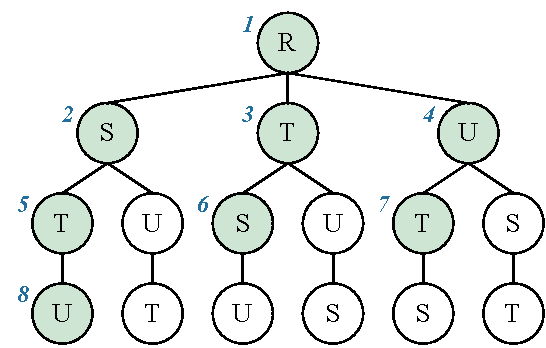
\includegraphics[width=0.6\linewidth]{figures/join_order_search_space.pdf}
    \vspace{-0.15cm}
    \caption{The Join Order Search Space as a Tree: A path from root to leaf denotes a sequence of joins. The visited nodes are marked in green, and the digits indicate the order in which they are visited using the Next-Best Join Order Search. At step 8, the algorithm emits the first join order $\langle R, S, T, U \rangle$.}
    \label{fig:search_space}
    \vspace{-0.3cm}
\end{figure}

\textbf{Pipeline Transformation:} Finally, we replace the existing operator pipeline with a POLAR pipeline consisting of the multiplexer, the set of join orders, and the adaptive union. Note that the individual join orders reuse the read-only hash tables of the build sides without redundant allocation. This transformation does not break the pipeline to prevent further materialization points and redundant multiplexing overhead. Other non-blocking operators (\eg projections, filters) and the pipeline sink (\eg an aggregation) also remain unchanged. The POLAR pipeline allocates space for state per alternative join order (e.g., operator caches, intermediate result vectors) instead of once. However, this space overhead is negligible since we limit the number of join orders for large queries.

\begin{algorithm}[!t]
\caption{Next-best Join Order Search}\label{alg:enumeration}
\begin{algorithmic}[1]
\Require{Joins $J$, Edge Counts $n_0, ..., n_{\card{J}} \in N$, Max Join Orders $\mathit{MAX}$}
\Ensure{Join Orders $T$}
\State $R \gets \emptyset$
\State $S \gets \textsc{LegalJoinCandidates}(R, J)$ \Comment{Find first join candidates}
\For{$i \gets 0$ \textbf{to} $n_0$}
    \Comment{Consider $n_0$ of the candidates}
    \State $s_i \gets \textsc{GetNextJoin}(S)$
    \State $\mathit{prio} \gets (\card{R}, i)$
    \State $pqueue.\textsc{Enqueue}(prio, R, s_i)$
    \State $S \gets S \setminus s_i$
\EndFor
\While{$!pqueue.\textsc{Empty}()$ and $\card{J} < \mathit{MAX}$}
    \State $R, s \gets pqueue.\textsc{Dequeue}()$ \Comment{Remove next item}
    \State $R \gets R \oplus s$
    \If{$\card{R} = \card{J} - 1$}
        \State $R \gets R \oplus J \setminus R$ \Comment{Append remaining join}
        \State $T \gets T \cup R$
    \Else
        \State $S \gets \textsc{LegalJoinCandidates}(R, J)$
        \For{$i \gets 0$ \textbf{to} $n_{\card{R}}$}
            \State $s_i \gets \textsc{GetNextJoin}(S)$
            \State $\mathit{prio} \gets (\card{R}, i)$
            \State $pqueue.\textsc{Enqueue}(prio, R, s_i)$
            \State $S \gets S \setminus s_i$
        \EndFor
    \EndIf
\EndWhile
\State \Return $T \cup \textsc{GetOriginalJoinOrder}()$
\end{algorithmic}
\end{algorithm}


\subsection{Join Order Selection}
\label{sec:paths}

When generating alternative join orders for individual pipelines, we aim to compose a diverse set of orders that could handle a wide range of mis-estimated cardinalities and cluster data. The selection strategy should be robust for very large pipelines (\ie find good plans early) and should not need to re-invoke the query optimizer~(\ie ensure non-invasive integration and low compilation overhead). To this end, we propose a set of simple join order selection strategies that only leverage previously estimated cardinalities. 

\textbf{Next-best Search:} Algorithm~\ref{alg:enumeration} shows our \emph{next-best search}. It uses a priority queue to explore join candidates, similar to a breadth-first search. The algorithm considers the search space a tree with nodes representing legal join sequences, while their children represent potential join candidates. In this tree, the set of all paths from root to leaf node represents the set of all legal join orders. Figure~\ref{fig:search_space} shows an example of such a join order search tree. We explore the tree by retrieving all possible join candidates $S$ for a given node representing a partial join sequence $R$. The function $\textsc{GetNextJoin(S)}$ then determines the $n_{\card{R}}$ fittest candidates, with $n_{\card{R}}$ being the number of edges to consider at a certain tree level. For each candidate $s_i$, the algorithm pushes an item containing the current node, the join candidate $s_i$, the tree level (\ie the length of the current join sequence $R$), and the fitness index $i$. The priority queue compares its items based on the tree level and fitness index---similar to recent heuristic search strategies in join enumeration to maximize pruning \cite{HaffnerD23}---so that the fittest join candidate in the lowest level is always the next item to retrieve. 
Depending on the values for $N=(n_0, \ldots, n_{\card{J}})$, the maximum number of join orders to generate $\textit{MAX}$, and the implementation of $\textsc{GetNextJoin}$, the algorithm allows finding different join order subsets. For example, setting $N$ to increasing values favors diversity of join candidate options for the rear joins of a join order, whereas decreasing values do the opposite. To keep the pipeline's space and exploration overhead manageable, we set $\mathit{MAX}$ to 24, which is high enough to exhaustively enumerate all join orders with five relations for clique queries (in general, $(n-1)!$, and thus, $(5-1)!=24$) and six relations for chain queries (in general, $2^{n-2}$, and thus, $2^{6-2}=16$)~\cite{MoerkotteN06}.
We implement three versions of the $\textsc{GetNextJoin}$ function:
\begin{itemize}
\item \textbf{S1 \textsc{GetRandom}:} Pick a random join candidate.
\item \textbf{S2 \textsc{GetMinCard}:} Pick the join candidate with the lowest estimated cardinality.
\item \textbf{S3 \textsc{GetMinCardUc}:} Pick the join candidate with the lowest, uncertainty-adjusted cardinality (every join has an uncertainty level derived from the number of preceding operators, assuming that the number of operators is correlated with potential misestimations, we multiply each candidate's cardinality estimate by its uncertainty level).
\end{itemize}

\textbf{Basic Heuristics}
Besides the search-based approach, we use two simple additional heuristics to generate alternative join orders: 
\begin{itemize}
\item \textbf{S4 \textsc{PushDown}:} Permute the original join order such that each join gets pushed to be the first in the join order once if legal (assuming that the first join in the pipeline often has the largest performance impact~\cite{DBLP:conf/damon/SchubertGZM23}).
\item \textbf{S5 \textsc{PullUp}:} Pull each join to the last position in the join order if possible (assuming that join blowups may be mitigated if the problematic join is pulled up to the end of the join order as other joins may filter its input).
\end{itemize}
We introduced these different join order selection strategies to allow for a systematic experimental evaluation, but by default, we employ \textsc{GetMinCard}, which provides robust characteristics in our experiments. Moreover, we set $N$ to be $\textsc{Min}(4 - \card{R}, 2)$ to favor diversity for the first few join options in the set of join orders.

\subsection{Pipeline Execution}\label{sec:execution}

During query execution, POLAR routes tuples from the source table of a pipeline through multiple join paths. The pipeline executor of these paths reports the performance and calculates their \emph{resistance} for future routing decisions. By using thread-local state (e.g., for tuple buffers and multiplexer state), POLAR can execute its pipelines in parallel without blocking. In this section, we discuss the related techniques for pipeline orchestration, our resistance metric, and parallel execution strategies in detail.

\textbf{Pipeline Orchestration:} To process a POLAR pipeline, the host database system spawns a custom POLAR pipeline executor responsible for passing tuples to the operators with respect to the multiplexer's routing decisions. 
The executor fetches chunks (\ie mini-batches or sets of tuples) from the source table and passes them sequentially through the pipeline. The multiplexer consumes a chunk and returns an output chunk containing a subset of the input (or the whole input) and the index of the next join order to pass the subset to. If the multiplexer does not return all tuples from the input, the executor re-invokes the multiplexer with the same input chunk in the next iteration to emit the next tuple subset instead of fetching a new chunk from the source. After routing the chunk to its dedicated join order, the executor passes the chunk to the adaptive union, other operators in the pipeline, and finally to the pipeline sink.
During this process, we count the number of intermediates appearing within the path as a performance indicator. We chose intermediate counts over clock time or CPU cycles because they allow an isolated observation of a single iteration (irrespective of other operators and parallelism), and the related $C_{out}$ cost model is known to be simple yet very accurate \cite{moerkotte23, LeisGMBK015}. Moreover, a clock time metric is biased towards paths receiving many input tuples as their throughput tends to be higher due to vectorization. After fully processing one multiplexer output chunk in a join order, the executor reports back the number of intermediates from that routing iteration to the multiplexer. This design allows adapting the \emph{plans of least resistance} to cluster data. For this reason, we currently never discard any of the join orders.

\textbf{Resistance Metric:} As a proxy for performance, the POLAR executor calculates a join order \emph{resistance}. This quantity comprises the sum of intermediate results $I$ observed in the current routing iteration, the number of tuples routed to the current join order $T$, and a constant $w$ representing the overhead of a routing iteration without intermediate results. We calculate the resistance $r$ as ${r = \frac{I}{T} + w}$. The overhead constant $w$ prevents edge cases of a routing iteration with zero intermediates per input counting as infinitely better than an iteration with one intermediate because there are still probing costs. If only a few tuples are routed to a join order, the resistance may not be representative for a larger set of tuples. Consequently, the executor applies a moving average from previous iterations for smoothing fluctuations.

\begin{figure}
    \centering
    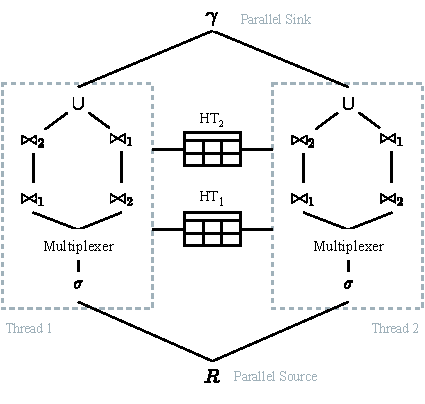
\includegraphics[width=0.9\linewidth]{figures/parallel-exec.pdf}
    \vspace{-0.5cm}
    \caption{Parallel Execution: Each thread processes a pipeline with an isolated state, sharing build sides to probe into.}
    \vspace{-0.25cm}
    \label{fig:parallel-exec}
\end{figure}

\textbf{Parallel Execution:} Similar to traditional data-parallel processing, POLAR executes pipelines in a multi-threaded fashion by starting multiple executors with thread-local states (cf. Figure~\ref{fig:parallel-exec}). The executors concurrently fetch batches of tuples from the pipeline source and push results to the sink. Each executor has an isolated multiplexer state and calculates the path resistances solely based on the tuples it has fetched. Note that the executors only isolate their processing states but share build-side data structures such as read-only hash tables. With the input tuples, the executor follows the paths sequentially and independently from each other. The lack of a global multiplexer state may delay routing decisions to better paths as each multiplexer must individually measure resistances before finding the next path. On the other hand, this parallel execution method avoids synchronization among the executors preventing wait time. As an alternative model for parallel processing to compare against, POLAR supports spawning one thread per join order and applying a backpressure mechanism to route tuples in a self-scheduling manner (cf. Section~\ref{sec:backpressure}).


%%%%%%%%%%%%%%%%%%%%%%%%%%%%%%%%%%%%%%%%%%%%%%%%%%%%%%%%%%%%%%%%%%%%%%%%%%%%%%%%%%%%
%% ROUTING STRATEGY
%%%%%%%%%%%%%%%%%%%%%%%%%%%%%%%%%%%%%%%%%%%%%%%%%%%%%%%%%%%%%%%%%%%%%%%%%%%%%%%%%%%%


\section{Routing Strategies}
\label{sec:routing_strategies}

At the core of POLAR pipelines is the multiplexer operator that makes routing decisions to determine the number of input tuples for each join order. To this end, the pipeline executor passes an input chunk (by default 1024 tuples) to the multiplexer, which uses a \emph{routing strategy} to return the next join path index and a subset of the tuples to route. The routing strategies attempt to follow the \emph{plans of least resistance}, which is the---potentially temporally changing---sequence of join order paths that incur the fewest number of intermediates. In this section, we first discuss the overall multiplexer algorithm, followed by four dedicated routing strategies used by the multiplexer and one self-scheduling strategy.

%%%%%%%
\subsection{Overall Multiplexer Algorithm}

Algorithm \ref{alg:multiplexer} shows the overall multiplexer algorithm. In the initialization phase, the multiplexer sends a small number of tuples to each join order with a resistance of zero (\ie an uninitialized join order without reported resistance) to measure initial performance. When all join orders are initialized, the multiplexer requests a tuple distribution from a configurable routing strategy. The distribution indicates the fraction that each join order receives from the current input chunk. The algorithm finally returns the join order index with the largest fraction and its respective input tuple count. If the multiplexer does not emit all tuples from the input chunk, the multiplexer emits the remaining tuples from the tuple distribution in the next iteration until the input chunk is fully processed (cf. Section~\ref{sec:execution}).
%
In the following, we introduce four different routing strategies implementing the tuple distribution method. Assuming that POLAR is executed in a vectorized database system, the implementation must trade-off path optimality (following the cheapest path through the join orders) and operator cache friendliness (minimizing the number of join order switches). The caching aspect can impact the processing performance as the pipeline executor must flush all operator caches buffering intermediates for vectorization before reporting the join order resistance to ensure that each input tuple has been fully processed and was thus correctly counted. Additionally, processing without buffering or too frequent plan switches may increase the number of instruction cache misses~\cite{SirinTPA16}. 

\begin{algorithm}[!t]
\caption{Multiplexer}\label{alg:multiplexer}
\begin{algorithmic}[1]
\Require{Tuple Distribution $T$, Resistances $\mat{W}$}
\Ensure{Join Order Index $\mathit{idx}$, Tuple count $c$}
\If{$\exists t_{\mathit{idx}} \in T: t_{\mathit{idx}} > 0$}
    \State $\mathit{fraction} \gets t_{\mathit{idx}}$ \Comment{Route tuples from previous multiplexing}
    \State $t_{\mathit{idx}} \gets 0$
    \State\Return $\mathit{idx}$, $\mathit{fraction} \cdot \mathit{INPUT\_SIZE}$
\ElsIf{$\exists w_{\mathit{idx}} \in \mat{W}: w = 0$} \Comment{Initialize join order}
    \State\Return $\mathit{idx}$, $\textsc{INIT\_COUNT}$
\EndIf
\State $T \gets \textsc{GetTupleDistribution}(\mat{W})$
\State $\mathit{idx}, \mathit{fraction} \gets \textsc{max}(T)$
\State $t_{\mathit{idx}} \gets 0$
\State\Return $\mathit{idx}$, $\mathit{fraction} \cdot \textsc{INPUT\_SIZE}$
\end{algorithmic}
\end{algorithm}

%%%%%%%
\subsection{Static Selection}

Static routing strategies, or path selection approaches, do not perform any exploration apart from initialization. For this reason, they are very simple to implement, and thus, we omit their pseudo-code of $\textsc{GetTupleDistribution}$ but provide high-level descriptions.

\textbf{R1 \textsc{InitOnce}:} This simple strategy retrieves the join order with the lowest resistance after the initialization phase and then routes every following chunk to that join order. \textsc{InitOnce} is extremely cache-friendly (i.e., in terms of tuple buffering in operator pipelines) because it requires no cache flushes until the end of the query. However, this strategy is prone to bad routing decisions if a join order only performs well for the first few tuples. Moreover, it is unable to find well-performing paths for pipelines with different join orders being the best choice for different clusters of data.

\textbf{R2 \textsc{Opportunistic}:} The \textsc{Opportunistic} routing strategy is similar to \textsc{InitOnce} but makes use of the resistance reports after routing each chunk. If the reported resistance of the current join order exceeds the resistance of another, it routes the next input chunks to that join order. This approach allows switching join orders if the previous order deteriorates. However, the decision is solely based on the resistance of a single join order and old initialization results of others, which may miss additional opportunities, such as better plans for clusters of data. Cache flushing is needed but can be reduced by only updating the resistance after every $n$ chunks, trading granularity with cache-efficiency.  

%%%%%%%
\subsection{Pro-active Exploration}

In order to enable robust pathfinding for complex paths and varying data characteristics, routing strategies must pro-actively explore alternative join orders. To this end, these strategies periodically route tuples to join orders that performed sub-optimal in the past. We introduce two strategies that both use the notion of an \textit{exploration budget}. This budget bounds the overhead we allocate for finding the optimal join path with minimal intermediate results. The two following strategies use the exploration budget to calculate a tuple distribution over the join orders producing additional intermediate results within that overhead based on the join order resistances measured so far.

\begin{algorithm}[!t]
\caption{GetTupleDistribution -- \textsc{AdaptTupleCount}}\label{alg:adapt_tuple_count}
\begin{algorithmic}[1]
\Require{Resistances $\mat{W}$}
\Ensure{Tuple Distribution $T$}
\State $T \gets \textsc{Initialize}(\card{\mat{W}}, 1)$
\State $\mat{W} \gets \textsc{SortInc}(\mat{W})$
\State $\mathit{cost} \gets \textsc{LastElement}(\mat{W})$
\For{$i \gets \card{\mat{W}} - 1$ \textbf{to} $0$}\Comment{Calculate distribution bottom-up}
    \State $\mathit{target} \gets w_i \cdot (1 + \textsc{BUDGET})$
    \State $\mathit{decrease} \gets \frac{w_i - \mathit{target}}{w_i - \mathit{cost}}$
    \For{$j \gets i+1$ \textbf{to} $\card{\mat{W}}$}\Comment{Adjust fractions to new target}
        \State $t_j \gets t_j \cdot \mathit{decrease}$
    \EndFor
    \State $t_i \gets 1 - \mathit{decrease}$
    \State $\mathit{cost} \gets \mathit{target}$
\EndFor
\State\Return $T$
\end{algorithmic}
\end{algorithm}

\begin{figure*}[!t]
    \centering
    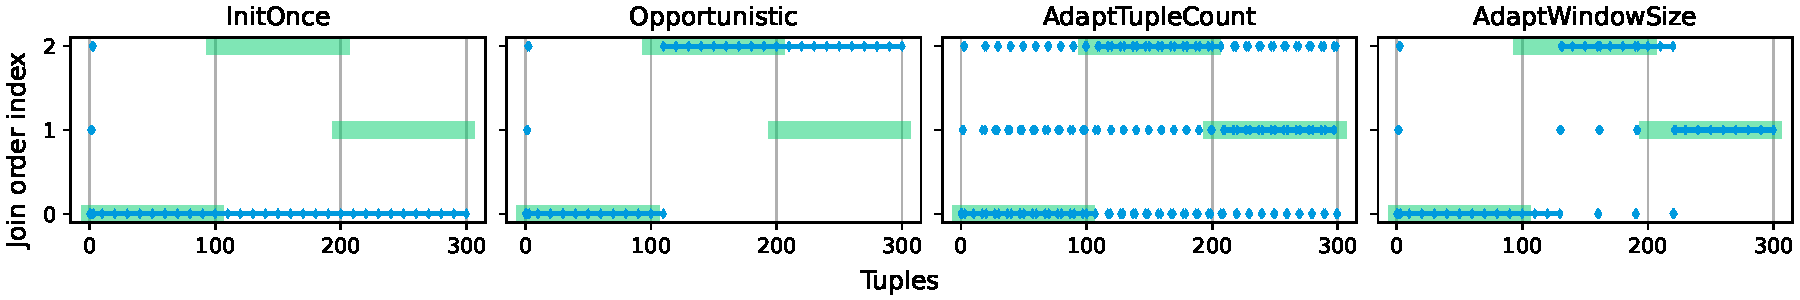
\includegraphics[width=\linewidth]{figures/routing_example.pdf}
    \caption{Behavior of four different routing strategies on an example scenario of 30 batches of 10 tuples each (green: optimal join paths, blue diamond: multiplexer invocations, blue line: path chosen by routing strategy).}
    \label{fig:routing_example}
\end{figure*}

\textbf{R3 \textsc{AdaptTupleCount}:} The \textsc{AdaptTupleCount} strategy (Algorithm~\ref{alg:adapt_tuple_count}) adapts the tuple allocation for each input chunk according to the exploration budget. This strategy initializes the output tuple distribution with ones (line 1), orders paths by their measured resistances (line 2), and adjusts the distribution in a bottom-up fashion. We start by reducing the problem to the two join orders with the highest resistances. The target cost is based on the lower resistance and the exploration budget, which we then use to calculate a \textit{decrease} factor (line 6). By multiplying that factor with the join order's tuple fraction (which was initialized to one), we find the amount of tuples that must be sent to the worst join order to stay within the exploration budget, based on the resistance of the second-last join order. Consequently, the amount for the second-last order is $1 - \mathit{decrease}$ (line 10). We calculate these values for the next-best join order while decreasing the fractions of the orders with higher resistances until we reach the first join order. \textsc{AdaptTupleCount} calculates tuple distributions for each incoming chunk, allowing for fine-grained path exploration bounded by the exploration budget. However, splitting each chunk into smaller sets of tuples obstructs vectorized execution and causes many cache flushes to report resistances. In our implementation, we only serve join orders receiving 64 or more input tuples to reduce the number of chunk splits. If a join order would receive less than 64 tuples, we redistribute those tuples to the other join orders. At the next multiplexer invocation, the implementation recalls those unserved tuples when calculating the next tuple distribution. 

\begin{algorithm}[!t]
\caption{GetTupleDistribution -- \textsc{AdaptWindowSize}}\label{alg:adapt_window_size}
\begin{algorithmic}[1]
\Require{Resistances $\mat{W}$}
\Ensure{Tuple Distribution $T$}
\State $T \gets \textsc{Initialize}(\card{\mat{W}}, 0)$
\State $t_{\textsc{minIndex}(W)} \gets 1$ \Comment{Route all tuples to least resistant order}
\State $\mathit{size}$, $\mathit{offset} \gets \textsc{GetWindowState}()$
\If{$\mathit{size} = 0$} \Comment{Determine window size}
    \State $W^{\prime} \gets \mat{W} \setminus \textsc{min}(\mat{W})$
    \State $\mathit{size} \gets \frac{1}{\textsc{INPUT\_SIZE}} \cdot \frac{\sum w^{\prime}_i \cdot \textsc{INIT\_COUNT}}{\textsc{BUDGET} \cdot \textsc{min}(W)}$
\EndIf
\If{$\mathit{offset} < \mathit{size}$}
    \State $\mathit{offset} \gets \mathit{offset} + 1$
\Else \Comment{Re-explore join orders next time}
    \State $\mat{W} \gets \textsc{SetToZero}(\mat{W} \setminus \textsc{min}(\mat{W}))$ \Comment{Reset resistances}
    \State $\mathit{offset}, \mathit{size} \gets 0$
\EndIf
\State $\textsc{SetWindowState}(\mathit{size}, \mathit{offset})$
\State\Return $T$
\end{algorithmic}
\end{algorithm}

\textbf{R4 \textsc{AdaptWindowSize}:} In contrast to \textsc{AdaptTupleCount}, the \textsc{AdaptWindowSize} strategy does not calculate individual tuple counts per join order. Instead, this strategy either routes complete chunks or a static, low number of tuples and adapts the window size (\ie number of input chunks) within which it will only serve the best join order. When exceeding the window, it re-initializes the remaining join orders by routing a small number of tuples to each of them. The internals of this strategy are shown in Algorithm~\ref{alg:adapt_window_size}, which distinguishes between three cases. Irrespective of the case, this strategy always returns a tuple distribution in which the best order receives the whole input chunk (line 2). If there is no window size calculated yet (line 4), we estimate the number of intermediates occurring in a reinitialization phase based on the resistances and adjust the number of tuples for reinitialization accordingly. We then divide the cost estimate by the overhead allowed by the exploration budget resulting in the number of tuples that should be routed to the best join order before reinitializing the others. The number of tuples per chunk scales this value down to the window size (line 6). If the current offset does not exceed the window size, we increment it (line~9). Finally, if the window size was exceeded, we set the resistances for all join orders---except the best---to zero (line 12) to trigger the initialization in the next multiplexer invocation. By routing multiple chunks to the same join order, the \textsc{AdaptWindowSize} strategy better allows for vectorization and can defer cache flushing until the window size is exceeded. On the other hand, its path exploration granularity is more coarse-grained than \textsc{AdaptTupleCount} as changes in resistances may appear within the routing window.

\begin{example2}[Routing Example] To illustrate the behavior of the four different routing strategies, Figure \ref{fig:routing_example} compares the multiplexer decisions for each of them in an example scenario. Given a POLAR pipeline with three join orders, 30 input chunks containing 10 tuples each. The resistances of the join orders change after every 10 chunks, namely $C_0 \gets \langle 1, 10, 15 \rangle$, $C_{10} \gets \langle 10, 15, 5 \rangle$, and $C_{20} \gets \langle 10, 1, 5 \rangle$. The resulting optimal path changes from the first to the third and then the second join order (indicated as green solid lines). The overlay blue diamonds show the multiplexer invocations of the different paths, and the blue line indicates the chosen path of least resistance. The \textsc{InitOnce} strategy tests every join order once in the beginning, then follows the optimal path temporarily but only until the 10th chunk. The \textsc{Opportunistic} strategy switches to the correct join order after the first one deteriorates but misses the second switch as it does not perceive the other join order's resistances. \textsc{AdaptTupleCount} correctly adapts to the optimal join paths but requires many switches and costly multiplexer invocations, including cache flushing. Finally, \textsc{AdaptWindowSize} first uses a large window so that it detects the join order switch only after a delay of a few chunks. Afterward, it reduces the window size as the difference between the resistances decreases. Therefore, the next switch comes after a shorter delay due to the finer granularity from the window resizing.
\end{example2}

\subsection{Self-scheduling}\label{sec:backpressure}

\textbf{R5 \textsc{Backpressure}:} To enable comparing against a self-scheduling strategy without parameters, we include a \enquote{backpressure} strategy. Instead of using a multiplexer, the POLAR pipeline spawns individual threads for each join order so that each thread concurrently pulls new input chunks. The approach does not depend on a budget and simply favors faster join orders as they can pull more chunks per time unit than others. The \textsc{Backpressure} strategy does not rely on multiplexing, does not require any operator cache flushes, and thus fully supports vectorized execution within each thread. However, with up to \textit{MAX} join orders (24 by default), this strategy has the intrinsic limitation that the majority of threads waste CPU cycles on sub-optimal join orders. 

%%%%%%%%%%%%%%%%%%%%%%%%%%%%%%%%%%%%%%%%%%%%%%%%%%%%%%%%%%%%%%%%%%%%%%%%%%%%%%%%%%%%
%% LIMITATIONS
%%%%%%%%%%%%%%%%%%%%%%%%%%%%%%%%%%%%%%%%%%%%%%%%%%%%%%%%%%%%%%%%%%%%%%%%%%%%%%%%%%%%

\section{Limitations}
\label{sec:limits}
%
POLAR is designed for adaptive query processing with non-invasive system integration as well as small and bounded overhead. This design leads to certain limitations as its applicability is ultimately dependent on the system's existing query optimizer. 
\begin{itemize}
\item \emph{Amenable Pipelines:} POLAR only replaces left-deep-trees. If the optimizer emits a right-deep tree (where intermediates feed into the build side of hash joins), POLAR cannot generate alternative join orders, as there are no pipelines with more than one join. Support for directed acyclic graphs (DAGs) and bushy trees is interesting future work.
\item \emph{Source Table:} As POLAR replaces normal operator pipelines that consume tuples from a specific source, it cannot change the source (sometimes called driver \cite{LiSMBCL07}) table.
\item \emph{Join Orders:} Our join order selection strategies use---except for uncertainty heuristics---only existing optimizer statistics. Thus, the alternative join orders could lack a well-performing join order for pipelines with many joins.
\item \emph{Operator Types:} So far, we only support pipelines with sequences of joins. Extended support for additional operators---such as projection, selection, and groupjoin \cite{MoerkotteN11}---is interesting future work as well.
\end{itemize}


%% EXPERIMENTS
\section{Experiments}
\label{experiments}

Our experimental evaluation of a prototype implementation of POLAR studies its general applicability and performance characteristics with a variety of benchmarks. After describing the prototype and experimental setting, we use various micro benchmarks to evaluate the behavior of different strategies and parameters and conduct end-to-end performance comparisons with DuckDB~\cite{RaasveldtM19}, Postgres~\cite{DBLP:conf/sigmod/StonebrakerR86}, and SkinnerDB~\cite{TrummerWMMJA19, TrummerWWMMJAR21} (as a representative AQP system). Our major findings are that: 
\begin{enumerate}
\item Non-invasive AQP yields robust end-to-end performance,
\item Offers substantial speedups for certain queries, especially on skewed benchmarks, and
\item Is already effective with small exploration budgets of $\leq$10\%. 
\end{enumerate}

\subsection{Experimental Setup}

\textbf{Prototype:} We implemented POLAR in DuckDB, a state-of-the-art OLAP DBMS. The prototype\footnote{On acceptance, we will share both the POLAR prototype implementation as well as scripts and artifacts of the experiments at \url{https://github.com/damslab/reproducibility}.} implementation, including several different routing and selection strategies, is ~2500 LoC and requires minimal changes to the existing DuckDB code. The input to the POLAR implementation is a query plan produced by the DuckDB optimizer, which uses equivalence sets to estimate cardinalities~\cite{thesis/Ebergen22} and the DPhyp~\cite{MoerkotteN08} algorithm to enumerate join orders.  

\textbf{Evaluation System:} We conducted all experiments on a Lenovo ThinkSystem SR635 server with a single AMD EPYC 7443P CPU at $2.85$\,GHz (24 physical/48 virtual cores), 256\,GB DDR4 RAM at 3.2\,GHz, $1\times 480\,\text{GB}$ SATA SSD, $8\times 2\,\text{TB}$ SATA HDDs (data) and Mellanox ConnectX-6 HDR/200\,Gb Infiniband. We compiled the source code with clang-12 on Ubuntu 20.04.1.

\textbf{Benchmarks:} We evaluate POLAR using the Join Order Benchmark (JOB)~\cite{JoinOrderBenchmark}, Star-Schema Benchmark (SSB)~\cite{SSB-ONeil2009-qs}, and a modified version of SSB including cross-correlation and skew (SSB-skew). We use both SSB versions with a scale factor of 10.
%
We introduce SSB-skew to evaluate how POLAR handles highly correlated and skewed data. This benchmark represents real-world data patterns and is very challenging due to cardinality estimation errors and non-uniform data clustering. SSB-skew introduces two new tables to SSB with n-to-m joins: \texttt{lineorder\_customer} and \texttt{lineorder\_part} with seasonal variance: \texttt{lineorders} may have multiple \texttt{customers} and \texttt{parts} if their order dates are within certain months each year. In other months, all \texttt{lineorders} have the same supplier. The \texttt{lineorder} table is ordered by order date. SSB-skew contains eight queries, each joining between 3 - 7 tables using a diverse set of predicates on the dimension tables.  % 
%
We considered TPC-H \cite{tpch} and JCC-H \cite{JCC-H} but did not use them because (1) their optimal join orders are well-known and often tuned for, and (2) the join orders generated by DuckDB are mostly right-deep trees which are not amenable to POLAR. We also considered the LDBC Social Network BI Workload~\cite{LDBC}, but LDBC requires advanced SQL features which are not supported by all systems we compare, and the DuckDB optimizer often generates pipelines with alternating joins and projections, which our prototype implementation does not yet support (cf. Limitations in Section~\ref{sec:limits}).
%

\subsection{Potential Benefit Analysis}
\label{sec:potential-analysis}

In a first series of experiments, we aim to understand the potential of POLAR pipelines by estimating the possible reduction in the number of intermediate tuples with optimal routing strategies. These results serve as a baseline---in terms of an upper bound---for later experiments evaluating the quality of POLAR routing strategies. Furthermore, we also examine the time per benchmark spent in amenable pipelines. Combining these measures allows estimating the ideal overall performance impact.

\textbf{Potential Reduction of Intermediates:} Table~\ref{tab:1_2_potential_savings} shows the potential performance improvements achievable with adaptive join order switching. We calculated the potential improvement by measuring the number of intermediate results for all amenable pipelines using DuckDB's default join order, the best static join order for each pipeline, and an estimated optimal routing strategy. We determined this optimal value using a multiplexer debugging mode, routing each input chunk to every legal join order and measuring the minimal number of intermediates.
%
Table~\ref{tab:1_2_potential_savings} shows that dynamic tuple routing strategies reduce the number of intermediates for all benchmarks but that the potential improvement over an ideal static join order is most significant with skewed datasets. For JOB, the best static join order produces 25.84\,M tuples compared to 107.49\,M tuples from DuckDB's default join order. Dynamic routing further improves this number to 16.92\,M tuples. This result shows that a better static join order could improve JOB to a large extent without dynamic join order switching at runtime. For SSB, neither join order switching nor better join orders considerably improve the number of intermediates. The best static join order produces 57.83\,M tuples, a moderate improvement over the 86.65\,M tuples in the default DuckDB plan, and dynamic routing makes only a slight additional improvement to 55.06\,M tuples. DuckDB's near-optimal plan for SSB is expected because the benchmark contains well-behaved FK/PK joins and uniform, non-skewed data. For SSB-skew, however, which lacks such schema information and uniform data, the potential for improvement is much higher. The default DuckDB join order produces 929.87\,M tuples, while the best static join order produces 688.90\,M tuples. Tuple routing improves this by more than an order of magnitude to 25.15\,M tuples. The routing performs so much better because no single join order can adapt to the changing data distributions while processing the clustered data. 

\begin{table}[!t]
	\centering 
	\caption{Intermediate Tuple Reduction and Coverage of Amenable Piplines -- Total number of intermediate tuples and fraction of total execution time spent in amenable pipelines.}
	\vspace{-0.3cm} \setlength\tabcolsep{5pt}
	\begin{tabular}{lrrrr}
		\toprule
		\textbf{Benchmark} & \textbf{DuckDB} & \textbf{Routing} & \textbf{Static} & \textbf{Coverage}\\
		\midrule
		JOB &     107.49 M &      16.92 M &      25.84 M & 37 \%\\
		SSB &      86.65 M &      55.06 M &      57.83 M & 68 \%\\
		SSB-skew &     929.87 M &      25.15 M &     688.90 M & 97 \%\\
		\bottomrule
	\end{tabular}
	\label{tab:1_2_potential_savings}
\end{table}


\textbf{Coverage of Amenable Pipelines:} Given DuckDB's default query plans, we measure each benchmark's total execution time and the time spent processing POLAR-amenable pipelines (\ie pipelines containing left-deep trees of two or more joins). Comparing the difference of these values yields the \textit{Coverage}, that is, the fraction of time spent in improvable pipelines. Note that the coverage also includes other operators from these pipelines, such as scans and aggregations, which POLAR cannot improve. The Coverage column in Table \ref{tab:1_2_potential_savings} shows that for JOB, DuckDB only spends 37\% of the processing time in POLAR-applicable pipelines. Consequently, almost two-thirds of the total execution time cannot be improved by POLAR. For SSB, DuckDB spends 68\% of the time in applicable pipelines, but many of them are dominated by large table scans, and the joins only account for a small portion of the time. For SSB-skew, DuckDB spends almost all of the execution time (97\%) in applicable pipelines and joins account for a large fraction of that time, providing substantial room for performance improvements.

\begin{figure}[!t]
    \centering
		\vspace{-0.1cm}
    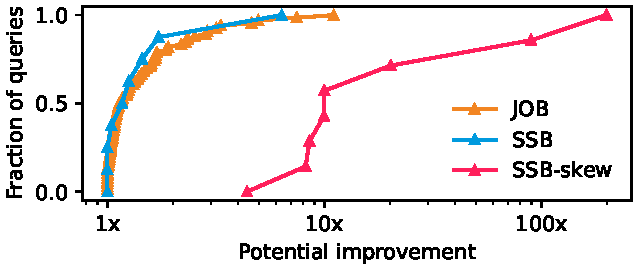
\includegraphics[width=\linewidth]{figures/1_3_potential_query_improvements.pdf}
    \vspace{-0.75cm}
		\caption{Potential Query Performance Improvement -- Estimated best case POLAR performance improvements.}
    \label{fig:1_3_potential_query_improvements}
		\vspace{-0.25cm}
\end{figure}

\textbf{Potential Query Performance Improvement:} Furthermore, we aim to assess how much the runtime of individual queries could be improved. We estimate these improvements per query by multiplying the optimal number of intermediates with the coverage of amenable pipelines (assuming a linear relationship between tuple count reduction and execution time). Figure \ref{fig:1_3_potential_query_improvements} shows a cumulative distribution function over the potential performance improvements for all queries. Some queries in both JOB and SSB can be improved by up to an order of magnitude. Queries in SSB-skew show a much larger potential for improvement: more than 50\% of queries can be improved by over an order of magnitude and some by up to 200x. 

\subsection{Micro Benchmarks}

\begin{figure*}[!t]
    \centering
    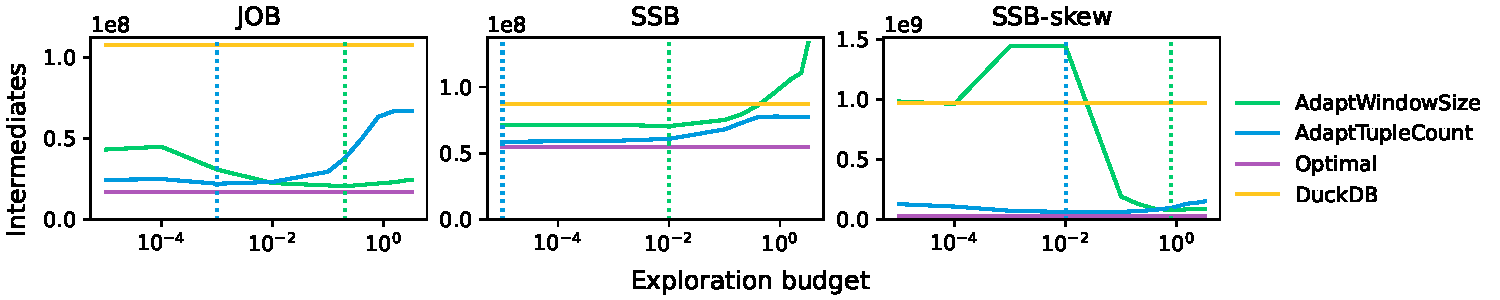
\includegraphics[width=\textwidth]{figures/2_3_routing_adaptive.pdf}
		\vspace{-0.75cm}
    \caption{Exploration Budgets -- Number of intermediate tuples for different exploration budgets. The dotted lines denote sweet spots in which the strategy generates minimal intermediates.}
    \label{fig:2_3_routing_adaptive}
\end{figure*}

To understand the trade-offs of different join selection and routing strategies, in a second series of experiments, we conduct several micro benchmarks regarding plan quality, compilation time, adaptivity, and runtime overhead. We also investigate the impact of the exploration budget on adaptivity and overhead. All micro benchmarks were executed single-threaded to isolate the effects.

\begin{table}[!t]
  \centering
  \caption{Join Order Selection -- Total number of intermediates for POLAR pipelines with different selection strategies.}
  \vspace{-0.3cm}  \setlength\tabcolsep{3.5pt}
  \begin{tabular}{lrrrr}
    \toprule
    \textbf{Enumeration} & \textbf{JOB} & \textbf{SSB} & \textbf{SSB-skew} & \textbf{JOB-ldt}\\
    \midrule
    DuckDB* &     107.49 M &      87.36 M &     967.78 M &     248.30 M\\
    Optimal &      16.92 M &      55.06 M &      25.15 M & N/A\\
    \midrule
    \textsc{GetRandom} &      16.92 M &      55.06 M &      25.15 M &     156.64 M\\
    \textsc{GetMinCard} &      16.92 M &      55.06 M &      25.15 M &     189.47 M\\
    \textsc{GetMinCardUc} &      16.92 M &      55.06 M &      25.15 M &     189.44 M\\
    \textsc{PushDown} &      17.04 M &      59.78 M &      41.46 M &     208.83 M\\
    \textsc{PullUp} &      17.22 M &      59.88 M &      53.08 M &     210.73 M\\
    \bottomrule
  \end{tabular}
  \label{tab:1_1_sel_intms}
\end{table}


\begin{figure}[!t]
    \centering \vspace{-0.1cm}
    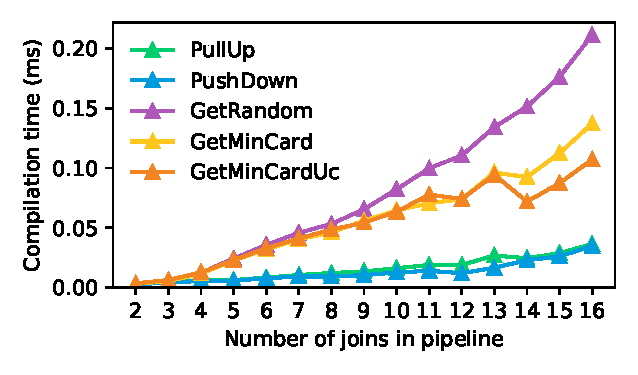
\includegraphics[width=\linewidth]{figures/2_2_enumeration_timings.pdf}
		\vspace{-0.75cm}
    \caption{Pipeline Compilation Time -- compilation time for join order selection strategies [milliseconds].}
    \label{fig:2_2_enumeration_timings}
		\vspace{-0.25cm}
\end{figure} 

\textbf{Join Order Selection:} We compare the quality of the join order selection strategies introduced in Section~\ref{sec:paths} by comparing the actual number of intermediates to the optimal number, as described in Section~\ref{sec:potential-analysis}. Table~\ref{tab:1_1_sel_intms} summarizes our findings. Since JOB, SSB, and SSB-skew only contain join pipelines with up to five relations, we can generate all possible join orders for these pipelines (cf. Section~\ref{sec:paths}). In order to stress test the different join order selection strategies, we also compared \textit{JOB-ldt}, which compiles the JOB queries using a greedy algorithm that only generates left-deep trees. For JOB and SSB, even simple strategies such as \textsc{PushDown} yield competitive results. However, for SSB-skew, the \textsc{GetRandom}, \textsc{GetMinCard}, and \textsc{GetMinCardUc} strategies produce substantially better join orders than the Default DuckDB plan because they are guaranteed to contain the optimal join order because they generate all possible candidates. For JOB-ldt, we observe that pure left-deep trees produce very large intermediates (273x larger) than a mix of bushy, left-deep, and right-deep trees. Interestingly, all join order selection strategies reduce the number of intermediates significantly (by more than 100x) but remain non-competitive compared to POLAR on top of DuckDB's default query optimizer.

\textbf{Pipeline Compilation Time:} The time required to compile a POLAR pipeline is dominated by the join order selection. We measured this compilation time for the join order selection strategies using pipelines with varying numbers of joins from JOB-ldt. Figure~\ref{fig:2_2_enumeration_timings} shows that the compilation time for \textsc{PushDown} and \textsc{PullUp} grows linearly with increasing number of relations, whereas the time of \textsc{GetRandom}, \textsc{GetMinCard}, and \textsc{GetMinCardUc} grows super-linearly. However, the absolute time required for any strategy---even for 16 joins---was less than one millisecond. Therefore, we conclude that the compilation time of POLAR pipelines is negligible compared to overall query processing times.

\textbf{Exploration Budgets:} For adaptive routing strategies, such as \textsc{AdaptTupleCount} and \textsc{AdaptWindowSize}, the quality of routing depends on the exploration budget. A higher budget allows the strategies to adapt better to path changes but also incurs larger overheads. To understand how the exploration budget affects the different workload characteristics, we execute JOB, SSB, and SSB-skew with exploration budgets from 0.001\% to 320\%. Figure \ref{fig:2_3_routing_adaptive} shows how the number of intermediates produced by the two adaptive routing strategies varies with increasing exploration budget. Both \textsc{AdaptTupleCount} and \textsc{AdaptWindowSize} achieve close to the optimal numbers of intermediates. However, the ideal exploration budgets differ for each benchmark. We attribute this effect to the differences in exploration potential, already observed in \ref{sec:potential-analysis}. While a larger budget only creates exploration overhead for SSB, such a budget is crucial to explore better join order alternatives for SSB-skew as the data distribution changes during query execution. \textsc{AdaptWindowSize} is especially sensitive to the exploration budget while \textsc{AdaptTupleCount} shows more robust behavior. Often, small exploration budgets of up to 10\% are sufficient to obtain robust performance characteristics. Moreover, the sweet spots for \textsc{AdaptWindowSize} are generally higher than for \textsc{AdaptTupleCount} as the latter consistently keeps exploring alternative join orders even under small exploration budgets.

\begin{table}[!t]
	\centering
	\caption{Intermediate Results -- Total number of intermediates per routing strategy using tuned exploration budgets.}
	\vspace{-0.3cm} \setlength\tabcolsep{7.9pt}
  \begin{tabular}{lrrr}
	\toprule
		\textbf{Routing Strategy} & \textbf{JOB} & \textbf{SSB} & \textbf{SSB-skew}\\
		\midrule
		DuckDB &     107.49 M &      86.65 M &     929.87 M\\
		Optimal &      17.01 M &      55.06 M &      25.15 M\\
        \midrule
		\textsc{InitOnce} &      43.27 M &      67.84 M &     985.83 M\\
		\textsc{Opportunistic} &      24.48 M &      58.71 M &     655.38 M\\
		\textsc{AdaptTupleCount} &      22.05 M &      \textbf{58.70 M} &      \textbf{62.93 M}\\
		\textsc{AdaptWindowSize} &      \textbf{20.51 M} &      70.53 M &     77.92 M\\
		\textsc{Backpressure} &      41.94 M &     227.33 M &     651.14 M\\
		\bottomrule
	\end{tabular}
	\label{tab:2_4_routing_all}
\end{table}


\textbf{Routing Strategies -- Intermediates:} We compare all routing strategies from Section~\ref{sec:routing_strategies} by the number of intermediate results they produce. For \textsc{AdaptTupleCount} and \textsc{AdaptWindowSize}, we set the exploration budgets according to the sweet spots found in the previous section. Table~\ref{tab:2_4_routing_all} shows that \textsc{AdaptTupleCount} performs robustly for JOB, SSB, and SSB-skew, whereas \textsc{AdaptWindowSize} produces the fewest intermediate results for JOB. \textsc{InitOnce} performs substantially worse than the adaptive strategies because it picks sub-optimal join orders whenever the initialization phase is not representative for the remaining data batches. This observation is especially pronounced for SSB-skew, where there are different optimal plans for different clusters of the data. \textsc{Backpressure} produces the most intermediate results because many executor threads process tuples in sub-optimal join orders.

\begin{table}[!t]
	\centering
	 \caption{Execution Time -- Total pipeline execution time per routing strategy [seconds].}
	 \vspace{-0.3cm}  \setlength\tabcolsep{11.4pt}
   \begin{tabular}{lrrr}
	  \toprule
		\textbf{Routing strategy} & \textbf{JOB} & \textbf{SSB} & \textbf{SSB-skew}\\
		\midrule
		DuckDB &      49.42 &       5.56 &      11.94\\
		\midrule
		\textsc{InitOnce} &      32.38 &       5.12 &      10.44\\
		\textsc{Opportunistic} &      31.44 &       6.78 &       9.40\\
		\textsc{AdaptTupleCount} &      31.44 &       7.46 &       6.50\\
		\textsc{AdaptWindowSize} &      31.02 &       5.21 &       5.36\\
		\textsc{Backpressure} &      68.35 &      14.26 &      20.65\\
		\bottomrule
	\end{tabular}
	\label{tab:3_1_pipeline}
\end{table}


\textbf{Routing Strategies -- Execution Time:} The performance of routing strategies does not solely depend on reducing intermediates. Another influential factor is how much adaptivity negatively affects vectorized execution. Tuple chunks produced by POLAR must contain vectors of sufficient size to amortize the per batch overheads, as explained in Section~\ref{sec:routing_strategies}. Therefore, we also examine the actual pipeline execution times for each routing strategy, as this is closely correlated to overall query execution time. Table \ref{tab:3_1_pipeline} shows the total pipeline execution time for different strategies, using the exploration budget sweet spots reported in the previous section. Since \textsc{AdaptWindowSize} trades path exploration granularity for better vectorization, the strategy performs best for exploration budgets that are below its sweet spots for minimal intermediates. Interestingly, the lowest number of intermediates does not necessarily lead to the lowest pipeline execution time. Despite creating substantially more intermediates, \textsc{InitOnce} performs competitively on JOB and outperforms the other strategies on SSB as it shows the cache-friendliest behavior. However, on SSB-skew, \textsc{AdaptWindowSize} has the lowest execution time and outperforms \textsc{InitOnce} substantially. \textsc{AdaptWindowSize} consistently performs better than \textsc{AdaptTupleCount}, despite creating more intermediates, which we attribute to \textsc{AdaptWindowSize}’s deferred cache flushing for sequences of routing decisions to the same join path. As \textsc{AdaptWindowSize} only performs slightly worse than \textsc{InitOnce} on SSB, we consider it to be the most robust routing strategy for the spectrum of workloads, achieving a good balance of reducing the number of intermediates and caching-friendly execution.

\begin{figure*}[!t]
    \centering
    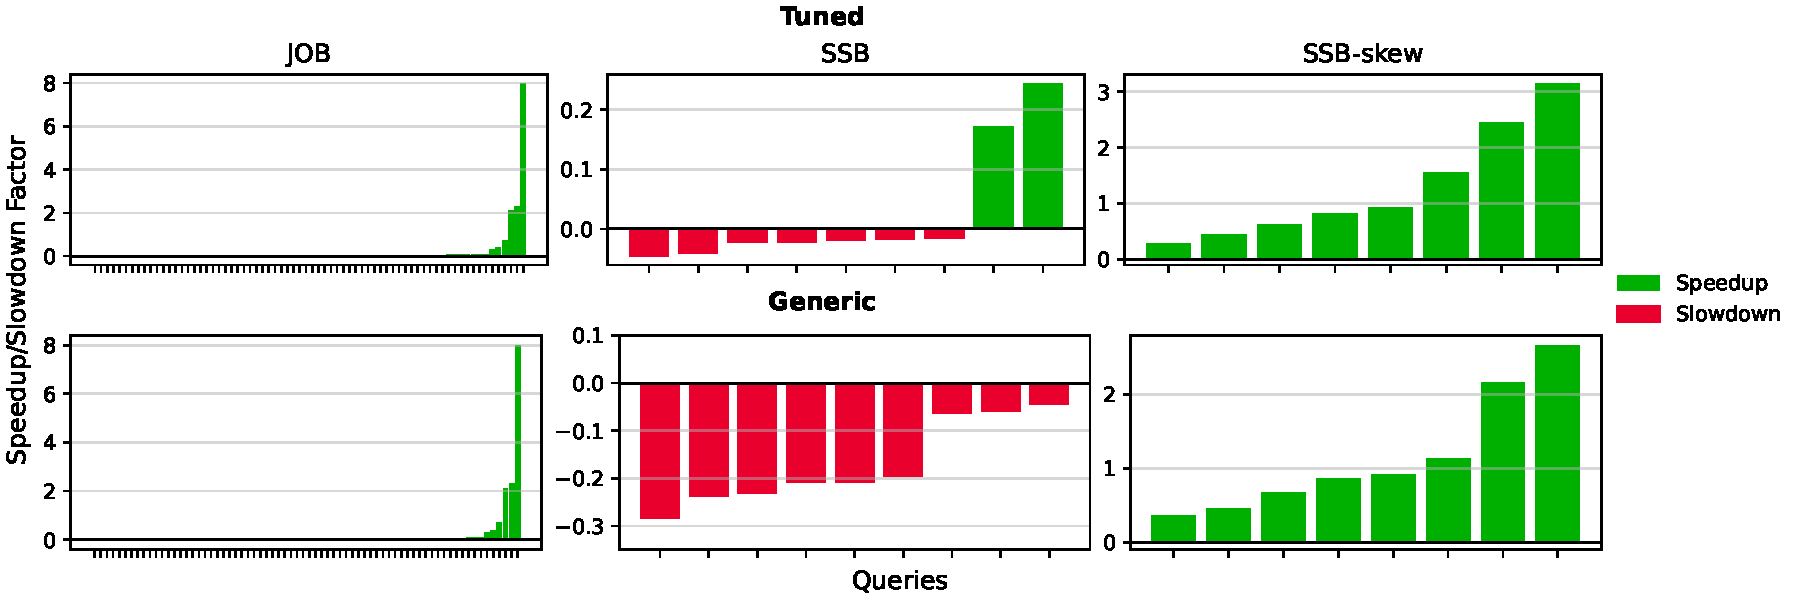
\includegraphics[width=\textwidth]{figures/3_2_rel_gains.pdf}
    \vspace{-0.55cm}
    \caption{Individual Query Performance Impact -- Query performance changes between unmodified DuckDB and POLAR. A value of +1 indicates the query was 100 \% faster (2x), and a value of -1 indicates a 100\% overhead (doubled execution time).}
    \label{fig:3_2_rel_gains}
\end{figure*}

\begin{table}[!t]
	\centering
	 \caption{Parameter Robustness -- Total pipeline execution time with generic vs. tuned exploration budgets [seconds].}
	 \vspace{-0.3cm}  \setlength\tabcolsep{8.7pt}
   \begin{tabular}{lrrr}
	  \toprule
		\textbf{Routing strategy} & \textbf{JOB} & \textbf{SSB} & \textbf{SSB-skew}\\
		\midrule
		DuckDB &      49.42 &       5.56 &      11.94\\
		\midrule
        \textsc{AdaptTupleCount} (0.01\%) &    32.73 &       7.60 &      6.84\\
		\textsc{AdaptTupleCount}-tuned &      31.44 &       7.46 &      6.50\\
        \midrule
		\textsc{AdaptWindowSize} (10\%) &      31.02 &       6.66 &       5.38\\
		\textsc{AdaptWindowSize}-tuned &      31.02 &       5.21 &       5.36\\
  		\bottomrule
	\end{tabular}
	\label{tab:3_3_parameter}
\end{table}


\textbf{Routing Strategies -- Parameter Robustness:} The previous experiment showed that routing strategies with tuned exploration budgets outperform static strategies for workloads on skewed, correlated data. However, it is not always possible to tune an exploration budget if the workload is unknown beforehand. For this reason, we evaluate the difference in execution times between a generic and tuned budget, summarized in Table~\ref{tab:3_3_parameter}. We compare the \textsc{AdaptTupleCount} and \textsc{AdaptWindowSize} routing strategies using their individual sweet spots to a static exploration budget that showed the best overall performance for JOB, SSB, and SSB-skew (0.01\% for \textsc{AdaptTupleCount}, 10\% for \textsc{AdaptWindowSize}). We observe that a generic exploration budget minimally increases execution times for \textsc{AdaptTupleCount} as this strategy generally has a robust performance for small budgets. In contrast, for \textsc{AdaptWindowSize}, a generic budget shows a larger deviation from its sweet spot for SSB but still performs better overall. Thus, we conclude that \textsc{AdaptWindowSize} is the preferable routing strategy despite its higher exploration budget sensitivity.

\subsection{End-to-End Performance Comparison}

Using the results from our micro benchmarks, we evaluate POLAR's end-to-end benchmark performance using \textsc{GetMinCard} join order selection, \textsc{AdaptWindowSize} routing strategy and both a generic 10\% exploration budget for all benchmarks (\textit{POLAR-G}), as well as tuned exploration budgets specific to each benchmark~(\mbox{\textit{POLAR-T}}), namely 10\% [JOB], 0.1\% [SSB], and 20\% [SSB-skew]. In this context, we compare POLAR with DuckDB~\cite{RaasveldtM19}, Postgres~\cite{DBLP:conf/sigmod/StonebrakerR86}, and SkinnerDB~\cite{TrummerWMMJA19}, a state-of-the-art AQP system, in both single- and multi-threaded configurations.

\begin{table}
	\centering
	\caption{Overall Performance Impact -- Single-threaded total execution time, and max execution time per query [seconds].}
		\vspace{-0.3cm} \setlength\tabcolsep{3.7pt}
   \begin{tabular}{lcccccc}
	  \toprule
		& \multicolumn{3}{c}{\textbf{Total Execution Time}} & \multicolumn{3}{c}{\textbf{Max. Query Time}}\\
         & JOB & SSB & SSB-skew & JOB & SSB & SSB-skew\\
		\midrule
		DuckDB & 135.5 & 7.8 & 12.2 & 10.7 & 1.1 & 3.6\\
        POLAR-G & 117.7 & 8.9 & 5.6 & 3.9 & 1.4 & 1.7\\
        POLAR-T & \textbf{117.7} & \textbf{7.5} & \textbf{5.6} & \textbf{3.9} & \textbf{0.9} & \textbf{1.7} \\
        Speedup & 1.15x & 1.04x & \textbf{\color{red}2.18x} & \textbf{\color{red}2.74x} & 1.22x & \textbf{\color{red}2.12x}\\
		\bottomrule
	\end{tabular}
	\label{tab:3_4_endtoend}
\end{table}


\begin{figure*}
    \centering
    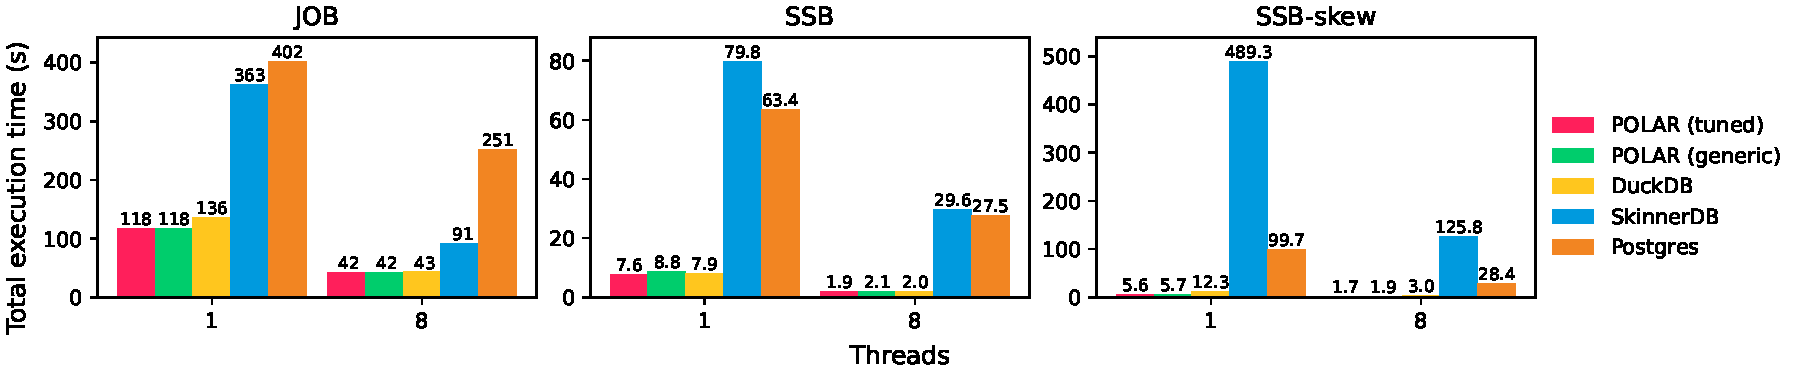
\includegraphics[width=\textwidth]{figures/4_1_total.pdf}
    \vspace{-0.55cm}
    \caption{AQP System Comparison -- Total execution times for JOB, SSB, and SSB-skew, using 1 and 8 threads [seconds].}
    \label{fig:4_1_total}
\end{figure*}

\textbf{Overall Performance Impact:} Table~\ref{tab:3_4_endtoend} shows the total end-to-end, single-threaded execution time---as well as the maximum query execution times---for DuckDB, POLAR-G, and POLAR-T on the different benchmarks. POLAR-T provides moderate total end-to-end performance improvements of 1.15x and 1.04x for JOB and SSB, respectively, and a substantial 2.18x end-to-end improvement for SSB-skew. Additionally, POLAR-T significantly improves the worst-performing queries by 2.74x in JOB, and 2.12x in SSB-skew. POLAR-G performs as well as POLAR-T for JOB and SSB-skew but shows more overhead on SSB. Generally, POLAR improves robustness by ensuring good execution time for all queries, even those where we would otherwise pick bad plans. 

\textbf{Individual Query Performance Impact:} Figure~\ref{fig:3_2_rel_gains} displays speedups and slowdowns for each query with POLAR-amenable pipelines in JOB, SSB, and SSB-skew. A value of 1 indicates an improvement of 100\% (\ie half the execution time or 2x), whereas a value of -1 indicates double the execution time. For most JOB queries, POLAR has no positive or negative effect on the execution time. However, for a few queries, POLAR substantially reduces the execution time by up to 9x. The two queries with the largest speedups are also the longest-running queries in the benchmark. On SSB, the POLAR overhead increases the execution time for most queries, as expected, given how close to optimal the original join plans are. POLAR's overhead is smaller than 5\% for any query when the exploration budget is properly tuned. With the generic configuration, POLAR's overhead is up to 28\%. Finally, all queries in SSB-skew improve with POLAR, up to 4x in some cases. Therefore, POLAR-T achieves substantial performance and robustness improvements with negligible overhead. With a generic budget, queries on uniform data may incur a perceivable overhead due to plan exploration and impact on vectorization at runtime. However, this moderate overhead is an acceptable price to pay for increased robustness, and the overhead could be further decreased when specializing POLAR to the underlying runtime characteristics.

\textbf{AQP System Comparison:} To contextualize POLAR's performance, we compare POLAR, DuckDB, Postgres, and SkinnerDB, measuring the total execution time in single- and multi-threaded (8 threads) configurations. We allow SkinnerDB to cache indexes on all join columns in memory to reduce its pre-processing time. We use Postgres 12.15 and set \texttt{max\_parallel\_workers\_per\_gather} to control the level of parallelism. Moreover, we disable nested-loop joins to prevent Postgres from choosing aggressive plans with fatal performance. Figure~\ref{fig:4_1_total} shows that with a tuned exploration budget, POLAR performs equally or better than DuckDB, SkinnerDB, and Postgres on all benchmarks and configurations. Using a generic exploration budget, POLAR performs slightly worse but still outperforms the other systems on JOB and SSB-skew. On SSB, the generic POLAR configuration performs worse than DuckDB for single-threaded but is comparable (2.1 vs 2.0 seconds) for multi-threaded execution. The increased parallelism seems to hide performance penalties from reduced vectorization opportunities. On SSB-skew, POLAR with both tuned and generic exploration budgets outperforms DuckDB by more than 2x single-threaded and more than 1.5x multi-threaded. SkinnerDB and Postgres both show much higher total execution times than POLAR and DuckDB, as expected, given their different target workloads and runtime systems. SkinnerDB performs worst on SSB and SSB-skew. On SSB (single- and multi-threaded) and SSB-skew (single-threaded), POLAR roughly outperforms SkinnerDB by 10x, whereas on multi-threaded SSB-skew, POLAR exhibits an improvement of 66-74x. We attribute this difference to the fact that SkinnerDB is restricted to choosing a single left-deep join plan and its non-vectorized execution. For SSB-skew, the uneven data distribution means any single join order, even if robust, can not capture the changing data skew over the course of the query's execution. Our performance experiments demonstrate the benefits of a non-invasive, bounded-overhead system design in an engine designed for analytic workloads. In contrast to invasive AQP systems, POLAR favors reusing existing database components and original plans resulting in competitive performance and much greater robustness with modest overhead.


%% RELATED WORK
\section{Related Work}
\label{related-work}
%
Besides the brief background on adaptive query processing and robust query processing in the introduction, here, we broadly survey related work and emphasize the differences of POLAR.

\textbf{Traditional AQP:} Adaptive query processing has received lots of attention in the data management literature, and great surveys \cite{BabuB05,DeshpandeIR07} and tutorials \cite{IvesDR07,DeshpandeHR06} already exist. Existing classifications distinguish AQP for traditional ad-hoc queries (or plan-based systems) versus continuous queries \cite{BabuB05}, as well as a spectrum of adaptivity from coarse- to fine-grained adaptation \cite{DeshpandeHR06}.
First, \emph{inter-query} optimization utilizes learned cardinalities for expressions \cite{BrunoC02,ChenR94,StillgerLMK01} for optimizing future queries. Second, \emph{inter-pipeline} optimization utilizes monitored statistics even within a single query. Examples are late binding (staged execution) with re-optimization at pipeline breakers \cite{DeshpandeHR06} or deferred parameter binding in parametric query optimization \cite{BizarroBD09}. Third, \emph{inter-operator} re-optimization compiles new remaining plans at so-called checkpoint operators \cite{KabraD98}. Similar, progressive and pro-active re-optimization apply plan changes if actual cardinalities are outside computed validity ranges \cite{MarklRSLP04,BabuBD05}. Fourth, \emph{intra-operator} adaptivity allows changing plans after partial operator evaluation. Examples are union stitch-up plans and handling of state in double-pipelined hash joins \cite{IvesHW04}, intra-query adaptivity via reinforcement learning in SkinnerDB \cite{TrummerWMMJA19,TrummerWWMMJAR21,WeiT22}, as well as adaptive join reordering of index-nested-loop joins with depleted states for correctness \cite{LiSMBCL07}. Fifth and finally, there is tuple routing with routing policies in Eddies~\cite{HellersteinA00,Arpaci-Dusseau03,Deshpande04,BizarroBDW05}. Many of these strategies require both optimizer and runtime extensions for effective and efficient adaptivity. Instead, POLAR aims at a simple system integration with bounded exploration overhead.

\textbf{AQP for Continuous Queries:} The adaptation of continuous queries---on conceptually infinite data streams---always focuses on \emph{intra-operator} and \emph{tuple-routing}. Early representative stream processing systems with adaptive query processing include STREAM \cite{BabuW04}, Aurora \cite{AbadiCCCCLSTZ03}/Borealis~\cite{AbadiABCCHLMRRTXZ05}, NiagaraCQ \cite{ChenJDTW00}, TelegraphCQ \cite{ChandrasekaranDFHHKMRRS03}, and others. Unique characteristics include the incremental collection of statistics to detect workload changes \cite{BabuMMNW04}, multi-query optimization with queries entering and leaving the system, the opportunity of asynchronous optimization outside the critical path \cite{Boehm2011}, applicability of load shedding \cite{TatbulCZCS03}, as well as stateful operators and queues which require draining during plan changes \cite{WangFMWZ19}. Modern distributed stream processing engines like Flink \cite{AlexandrovBEFHHKLLMNPRSSHTW14}, Spark \cite{ZahariaDLHSS13}, Beam \cite{AkidauBCCFLMMPS15}, Heron~\cite{KulkarniBFKKMPR15}/Dhalion~\cite{FloratouAGRR17}, and NebulaStream \cite{ZeuchCMGGGBTM20} further deal with the reconfiguration of distributed query topologies. In contrast to POLAR, AQP is naturally deeply integrated in almost all components of such stream processing engines.

\textbf{Different Plans for Different Data:} Both, ad-hoc and continuous queries are typically only compiled and optimized according to average statistics for entire tables. However, especially in correlated data, relations are naturally divided into partitions with different characteristics \cite{TzoumasDJ10}. Early work on selectivity-based partitioning \cite{Polyzotis05} and content-based routing \cite{BizarroBDW05} address this observation by generating different plans for different partitions (combined with union) and different value-based routing policies, respectively. Such approaches often leverage more fine-grained statistics such as serial histograms (i.e., detailed frequency matrices) \cite{Ioannidis93}. Recent work on multi-way join size estimation \cite{MullerM22,IzenovDRS21} utilize hash-based translation grids \cite{MullerM22} and AKMV sketches \cite{BeyerHRSG07} as well as fast-AGMS sketches \cite{IzenovDRS21}. Since selectivity-based partitioning might compute the same intermediate multiple times, further work on sharing-aware horizontal partitioning \cite{TzoumasDJ10} introduced a conditional join plan, and related optimization and runtime techniques. Exploratory AQP via reinforcement learning like SkinnerDB~\cite{TrummerWMMJA19} would also lend itself to discovering different paths. Due to repeated path sampling, POLAR can also exploit different paths for different data, but only if these tuples are scanned in a clustered manner.

\textbf{Micro Adaptivity:} Besides finding alternative plans (e.g., join orders), some work also focused on micro adaptivity. Raducanu et al. introduced this concept in Vectorwise \cite{RaducanuBZ13} by providing alternative kernel implementations (e.g., branch, no-branch), measuring their runtime on sample vectors, and selecting the best configuration via a learning algorithm. Later work used performance counters to minimize the measurement overhead, and more properties such as sortedness and co-clustering \cite{ZeuchPF16}. Other forms of micro adaptivity are compiling continuous queries for HW specialization, parallelization, as well as exploitation of selectivities or value ranges/distributions \cite{GrulichBZTBCRM20}. Although these techniques are very valuable, they require specific optimization algorithms, whereas POLAR by-design relies on existing optimizers without changes. 

\textbf{AQP for Non-relational Workloads:} Ideas from adaptive query processing have also been applied and extended for systems dealing with non-relational workloads. Examples include JIT compilation for programming languages~\cite{HolzleU94} (e.g., Java or WebAssembly); lazy expression compilation in TensorFlow~\cite{MoldovanDWJLNSR19}, dynamic recompilation of basic blocks and functions in SystemML~\cite{BoehmBERRSTT14}; periodic or on-demand reoptimization of message-oriented integration flows \cite{Boehm2011}; and adaptive query processing on RAW data \cite{KarpathiotakisBAA14}. These systems also incrementally collect telemetry and perform plan adaptation, but unlike POLAR, seek a new optimal plan or configuration. 

\textbf{Learned Optimizers and Estimators:} With the trend towards ML for systems---following the influential learned indexes work \cite{KraskaBCDP18}---there has been substantial progress on improved cardinality estimates that could mitigate some of the need for AQP. Early work focused on the featurization of schemas and workloads and sampling-based training data collection \cite{KipfKRLBK19,DuttWNKNC19,YangLKWDCAHKS19}. Hilprecht and Binnig later introduced representations for zero-shot cost models \cite{HilprechtB22,HilprechtB22b} that can generalize to unseen database instances. Early work like LEO \cite{StillgerLMK01} also focused on learned cardinalities, but in retrospective had the problem of "fleeing from knowledge to ignorance" \cite{Lohman17} because the exponential search space gets only sparsely sampled and skewed cardinalities are often larger than the estimates under independence assumption. However, recent work has shown that learned optimizers and cardinality estimators can learn from mistakes \cite{MarcusNMZAKPT19,MarcusNMTAK21}, making a case for stateful, learning-based systems \cite{abs-2303-15308}, especially in the context of cloud DBMS like Snowflake \cite{DagevilleCZAABC16} or Redshift \cite{GuptaATKPSS15}. In contrast to POLAR, integrating learned optimizers and estimators is still very invasive in terms of system complexity, bootstrapping process, and integration points.


%% CONCLUSIONS
\section{Conclusions}
% summary
We introduced the new concept of plans of least resistance for leveraging adaptive query processing in a non-invasive manner. POLAR pipelines replace, where applicable, standard join pipelines and internally multiplex tuple batches among alternative join paths. This design allows periodically sampling join paths, collecting telemetry, and adapting the routing to the best path accordingly. 
% conclusions
We draw three key conclusions. First, the simple design without optimizer changes greatly simplified the integration into systems such as DuckDB. Second, POLAR shows robust performance but only on workloads yielding a large fraction of applicable pipelines. Third, there are examples of substantial performance improvements for individual pipelines, queries, and workloads, especially for skewed data (fix for bad cardinality estimates) and clustered data (exploit different plans for different data partitions).
% future work
Interesting directions of future work include more advanced strategies for selecting alternative pipelines (e.g., considering the uncertainty of cardinality estimates), and broader support for different plan structures (e.g., DAGs, bushy plans, additional operators like groupjoin \cite{MoerkotteN11}). 


\begin{acks}
We thank the participants of Dagstuhl Seminar 17222~\cite{DBLP:journals/dagstuhl-reports/Borovica-GajicG17} and 22111~\cite{DBLP:journals/dagstuhl-reports/Borovica-GajicG22} for inspiring this research and invaluable discussions. We also thank SAP for funding this project.
\end{acks}

%\clearpage
\balance
\bibliographystyle{ACM-Reference-Format}
\bibliography{sample-base}

\end{document}
\endinput
